\documentclass{article}

\usepackage{graphicx}
\usepackage{amsmath}

\begin{document}

\title{All About Suicide Burns}
\maketitle

\begin{figure}[h]
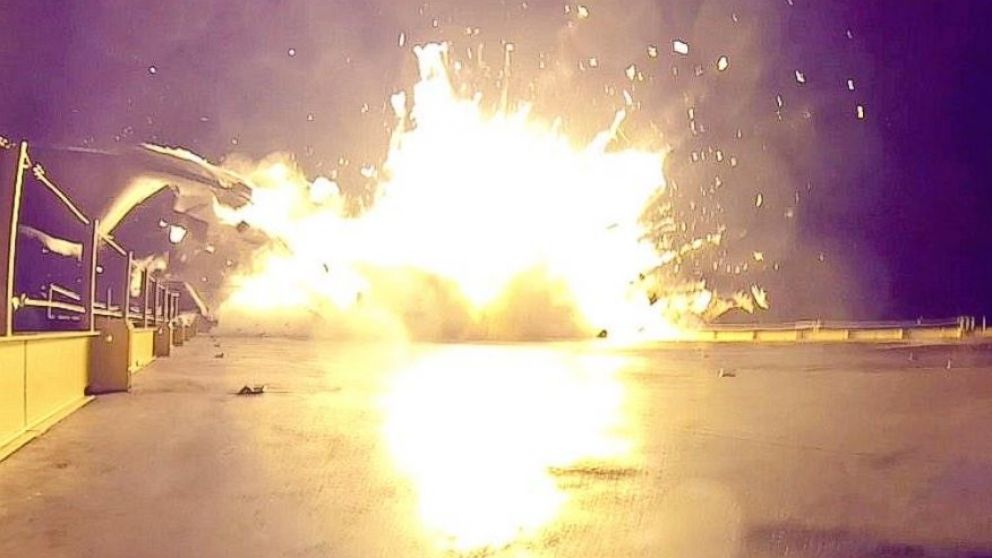
\includegraphics[width=0.8\textwidth]{falcon_9_barge_crash.jpg}
\caption{Unsuccessful Attempt at a Suicide Burn Landing by SpaceX}
\end{figure}

\section{Introduction}

Landing rockets is difficult, as evinced by the recent failures and 
	celebrated successes of SpaceX in landing an orbital first stage.
It is also a necessary part of a cost-effective re-usable rocket system.
The primary role of the first stage of an orbital rocket is to give as much
	speed and altitude as possible to the second stage, so that it can achieve
	orbit.
The first stage is therefore traveling extremely fast after releasing the second stage,
	so fast that experiments with parachute recovery have all ended in failure.
SpaceX and Blue Origin have recently tried a new approach:
	they use the rocket engines already on board the second stage to slow the
	rocket down for a soft landing.

If one is trying to land a rocket, one must first apply thrust to cancel out 
	any horizontal velocity with respect to the surface one is landing on.
Then, one needs to orient the rocket with its engine facing downwards, in the same
	position that it launched in, except moving the opposite direction.
Finally, one must fire the engines in order to slow down the rocket, so that
	it comes to a stop just as its landing legs begin to touch the ground.

One strategy for landing rockets is to wait as long as possible to fire the
	engines, firing them at the last possible moment and at full thrust.
This method, known as a ``suicide burn'' uses the least fuel, although it 
	is difficult to control for errors, since there is a very small margin for error.
To execute a sucide burn, the rocket only needs to know at what altitude to fire the
	engine so that it will come to a stop.
It can be necessary since it is difficult to design rocket engines which
	can throttle to less than half of their maximum thrust, and therefore 
	many rockets (such as SpaceX's
	Falcon 9) are unable to hover, because they can't apply 
	a \emph{small} enough force.
In this case, a suicide burn is the only option.

I will discuss techniques for planning suicide burns for two scenarios.
In both scenarios, the gravity is assumed to be of constant strength.
This is a valid approximation when close to the surface of a planet.
Since our rockets typically fire below 10km altitude for earth landings,
	we can safely use this approximation, which greatly simplifies
	calculations because the gravitational acceleration is now constant.
In the first scenario, the rocket applies a set force to itself with the engine,
	and its mass is fixed (i.e., no propellant is consumed).
This approximation is valid for slow landings, or landings which do not 
	consume an appreciable fraction of the mass of the entire rocket
	in fuel.
The second scenario takes into account the use of the fuel, and is therefore
	valid for faster landings.
I will discuss the differences between the predictions of the two models.
For each model, I will discuss how to determine the altitude at which
	to begin the deceleration burn.

\section{Model 1: Negligible Fuel Consumption}

This model will start by determining the motion of the rocket both while
	the rockets are on and off.
I will next determine how much distance a rocket will need to stop, if it is
	moving at a given velocity $v_0$.
Finally, I will use the freely-falling motion model to predict at what altitude
	to begin the burn.

\subsection{Determining Accelerations}

This model assumes that for the duration of the burn, 
	the rocket's mass has an approximately constant value, $m$.
When the rockets are not firing, the acceleration is entirely due to gravity,
	and is $-g$.
When the rockets are firing with force $F$, they exert an acceleration
	of magnitude $F / m - g$.

\subsection{Determining Stopping Distance}

If the rocket is moving with speed $v_0$ at the moment it fires its engines,
	then its distance and velocity from the point of initial firing will be:

\begin{align*}
	d(t) & = v_0 t + 1 / 2 a t^2 \\
	v(t) & = v_0 + a t \\
\end{align*}

When $v(t) = 0$, the rocket has stopped.
Therefore, the rocket stops at time:

\begin{align*}
	t_\text{stop} & = \frac {-v_0} a
\end{align*}

At that time, its distance from the point of initial firing is:

\begin{align*}
	d(t_\text{stop}) & = 
	v_0 \left( \frac {- v_0} a \right)
	+ \frac 1 2 a \left( \frac {-v_0} a \right)^2\\
	d(t_\text{stop})
	& = \frac {- v_0^2}	{2 a}
\end{align*}

Thus, if the rocket is moving at a speed $v_0$,
	it will take a distance $\frac {v_0^2} {2 a}$ to stop.

\subsection{Determining Firing Altitude}

When falling, the pilot should ignite the rocket when their altitude
	is equal to the stopping distance.
In this subsection we will determine what altitude this will be,
	given the altitude and vertical velocity of the rocket.

Solving for the $t$ such that $d(t) = x(t)$,
	we find:

\section{Model with Fuel Consumption}

In the previous model, we assumed that the rocket's mass is essentially
	constant for the duration of the burn.
If a rocket is attempting to land at high velocities, it will need to
	burn a significant fraction of its mass in propellant.

\subsection{Fuel Consumption}

The rocket's mass is assumed to be $m_0$ before the burn begins.
The rocket's engine, when operating at thrust $f$, will consume fuel
	at a constant rate $b$.
Therefore, the mass of the rocket is given by:

\begin{align}
	m(t) & = m_0 - b t
\end{align}

as long as $t$ is small enough so that the rocket does not use up all its fuel.

\subsection{Forces on the Rocket}

When the engine is not firing, the only force acting upon the rocket is gravity.
This force causes a downwards acceleration of magnitude $g$.

When the engine is firing, gravity and thrust are acting upon the rocket
	and together cause an acceleration of $f / m(t) - g$ at time $t$.

\subsection{Velocity of the Rocket Under Power}

Suppose the rocket is at an altitude $x_0$ and traveling with speed $v_0$,
	with none of its fuel consumed.
At time $t=0$, it ignites its engines.
Then, the velocity evolves according to the following 
	differential equation:

\begin{align}
	\frac {dv}{dt} (t) & = \frac f {m(t)} - g
\end{align}

This has the following solution which satisfies the boundary conditions:

\begin{align}
	v(t) & = v_0 - g t + \frac f b \log \left( \frac {m_0} {m_0 - b t} \right)
\end{align}

\subsection{Stopping Time}

To determine the time until the rocket comes to a stop, we need to solve
	the equation $v(t) = 0$ for $t$.
This is difficult to express analytically, however, numerical methods exist
	to find the solution.
The velocity as a function of time can be expanded to the second order about
	the origin, and this will provide an accurate initial guess for a numerical
	method such as newton's method.

At the origin, the acceleration is $\frac f {m_0} - g$, and the jerk is:

\begin{align}
	j(t) & = \frac {f b} {(m_0 - b t)^2} \nonumber \\
	j(0) & = \frac {f b} {m_0^2}
\end{align}

Therefore, the velocity as a function of time is approximately:

\begin{align*}
	v(t) & \approx v_0 + \left( \frac f {m_0} - g \right) t
		+ \frac {f b} {2 m_0^2} t^2
\end{align*}

and in this approximate expression, $t_\text{stop}$ is given by the solution
	to the equation:

\begin{align*}
	0 & \approx v_0 + \left( \frac f {m_0} - g \right) t
		+ \frac {f b} {2 m_0^2} t^2
\end{align*}

Solving this equation, we obtain the following approximate expression for $t_\text{stop}$:

\begin{align}
	t_\text{stop} & \approx	\frac{\sqrt{a(0)^2 + 2 j(0) (v_f - v_0)} - a(0)}{j(0)}
\end{align}

This guess can be improved by iterative procedures such as newton's method.
Note that if there is a propellent mass $m_p$ onboard, $b t_\text{stop}$ must be
	less than or equal to $m_p$.
If it is not, then the rocket will not be able to stop itself.

\subsection{Stopping Distance}

In order to know the distance the rocket takes to decelerate to a stop,
	one needs to determine the rocket's position of a function of time.
Fortunately, this is only as difficult as integrating the expression for the velocity.
The result is shown below:

\begin{align}
	x(t) & = x_0 + v_0 t - \frac 1 2 g t^2 + \frac f b \left[
		b t - \left(m_0 - b t\right) \log \left( \frac {m_0} {m_0 - b t} \right) \right]
\end{align}

Therefore, the distance required to stop, if moving at speed $v_0$, 
	is, if $v(t_\text{stop}) = 0$:

\begin{align}
	d_\text{stop} & = v_0 t_\text{stop} - \frac 1 2 g t_\text{stop}^2 
	+ \frac f b \left[ 
		-(m_0 - b t_\text{stop}) \log \left( \frac {m_0} {m_0 - b t_\text{stop}} \right)
		+ b t_\text{stop} \right]
\end{align}

\subsection{Burn Altitude}

We can finally solve the original problem from here:	
	given a rocket's initial position and velocity, find at what
	time and altitude it needs to burn at.
The burn will start at a time $t_\text{fire}$ from the initial time $t=0$.
At $t_\text{fire}$:

\begin{align}
	x(t_\text{fire}) & = d_\text{stop}(v(t_\text{stop}))
\end{align}

We must determine $t_\text{fire}$.



\end{document}

 
